\part{从一道简单而基础的数学题出发}
\section{平面中求面积}
我们先来看这样一道题目:

\begin{figure}
  \centering
  % Requires \usepackage{graphicx}
  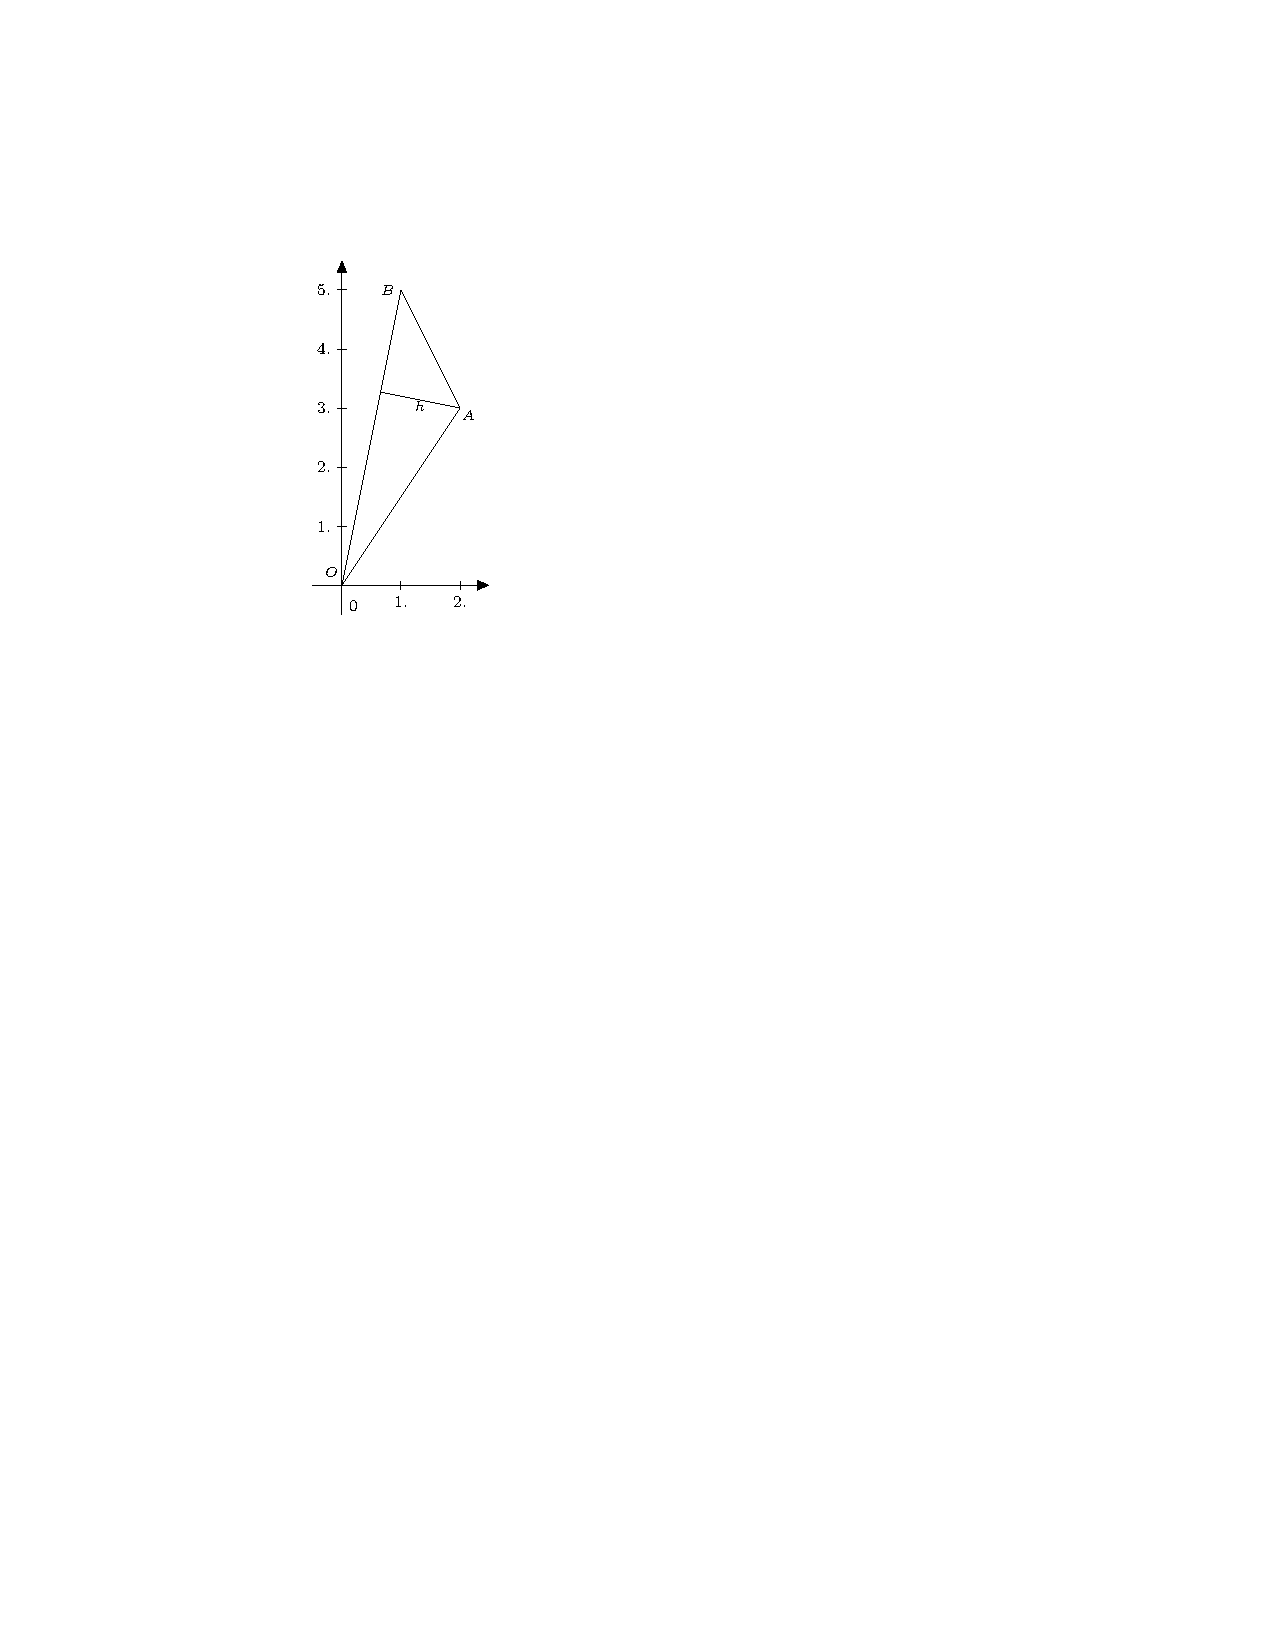
\includegraphics[width=3cm]{pic//1//1.pdf}\\
  \caption{一道简单而基础的数学题}\label{pro1}
\end{figure}

  \prob 如图\ref{pro1},在平面直角坐标系中,已知$A(2,3)$,$B(1,5)$,求$S_{\triangle ABO}$\\
\from{冯易}
  $\dps\because O(0,0),B(1,5)\\
  \so OB:5x-y=0;\textrm {又} A(2,3)\\
  \so OB\textrm{边上的高}h=\frac{\abs{10-3}}{\sqrt{5^2+1^2}}=\frac{7}{\sqrt{26}},
  \textrm{底边}OB=\sqrt{(1-0)^2+(5-0)^2}=\sqrt{26}\\
  \so S_{\triangle ABO}=\frac{1}{2}OB\times h=\frac{7}{2}$

考虑它的一般情况:

\prob 已知三点$A,B,C$,坐标分别为$(x_i,y_i),i=1,2,3$,求$S_{\triangle ABC}$\\
\from{冯易}
  $\dps\because A(x_1,y_1),B(x_2,y_2)\\
  \so AB:(y_1-y_2)x-(x_1-x_2)y+(x_1y_2-x_2y_1)=0;\textrm {又} C(x_3,y_3)\\
  \so AB\textrm{边上的高}h=\frac{\abs{(y_1-y_2)x_3-(x_1-x_2)y_3}}{\sqrt{(y_1-y_2)^2+(x_1-x_2)^2}},
  \textrm{底边}AB=\sqrt{(x_1-x_2)^2+(y_1-y_2)^2}\\
  \so S_{\triangle ABO}=\frac{1}{2}\frac{\abs{(y_1-y_2)x_3-(x_1-x_2)y_3+(x_1y_2-x_2y_1)}}{\sqrt{(y_1-y_2)^2+(x_1-x_2)^2}}\times \sqrt{(x_1-x_2)^2+(y_1-y_2)^2}\\
  =\frac{1}{2}\abs{(y_1-y_2)x_3-(x_1-x_2)y_3+(x_1y_2-x_2y_1)}\\
  =\frac{1}{2}\abs{x_1y_2-x_1y_3+x_2y_3-x_2y_1+x_3y_1-x_3y_2}
  $

本着对称轮换、简单优美的原则,我们有$$S_{\triangle ABC}=
\frac{1}{2}\left|\left|\begin{array}{ccc}
    1 & 1 & 1 \\
    x_1 & x_2 & x_3 \\ 
    y_1 & y_2 & y_3 
  \end{array}\right|\right|
  =
\frac{1}{2}\left|\left|\begin{array}{cc}
    x_2-x_1 & y_2-y_1 \\
    x_3-x_1 & x_3-y_1 
  \end{array}\right|\right|
  =\frac{1}{2}\abs{\vv{AB}\times\vv{AC}}
$$

\section{空间中求体积}

\prob 在空间直角坐标系中,已知四点$A,B,C,D,\textrm{坐标为}(x_i,y_i,z_i)(i=1,2,3,4)$,求$V_{\textrm{三棱锥}A_1A_2A_3A_4}$(以下简写为$V$)

\from{冯易}首先我们有
\begin{eqnarray}
V&=&\frac{1}{3}S\cdot h\nonumber
\end{eqnarray}
而
\begin{eqnarray}
S&=&\frac{1}{2}\left |\vv{AB}\times \vv{AC} \right|\nonumber\\
h&=&\left|\vv{AD} \right| \cdot \cos<\textrm{面ABC,直线AD}>\nonumber
\end{eqnarray}
注意到
\begin{eqnarray}
\cos<\textrm{面ABC,直线AD}>=\left|\cos<\vv{AB}\times \vv{AC},\vv{AD}>\right|\nonumber
\end{eqnarray}
故
\begin{eqnarray}
\label{equtionOfV}
V=\frac{1}{6}\left|\left(\vv{AB}\times\vv{AC}\right)\cdot\vv{AD} \right|
\end{eqnarray}
在式(\ref{equtionOfV})中用到了向量的数量积和向量积,$(\bm{a}\times\bm{b})\cdot\bm{c}$ 称为(向量)$\bm{a},\bm{b},\bm{c}$的混合积\footnote{不严谨的定义}

建立标准单位向量\footnote{
  未作特别说明,分别以$\bm{i},\bm{j},\bm{k}$记$x$轴,$y$轴,$z$轴上与该轴正向同方向的单位向量
  }
  $\bm{i},\bm{j},\bm{k}$, 将向量用坐标表示
\begin{eqnarray}
\vv{AB}&=&(x_2-x_1,y_2-y_1,z_2-z_1)\nonumber\\
\vv{AC}&=&(x_3-x_1,y_3-y_1,z_3-z_1)\nonumber\\
\vv{AD}&=&(x_4-x_1,y_4-y_1,z_4-z_1)\nonumber
\end{eqnarray}
则
\begin{eqnarray}
\vv{AB}\times\vv{AC}&=&
(x_2-x_1,y_2-y_1,z_2-z_1)\times(x_3-x_1,y_3-y_1,z_3-z_1)\nonumber\\
\label{crossProduct}
&=&\left|
  \begin{array}{ccc}
    \bm{i} & \bm{j} & \bm{k} \\
    x_2-x_1 & y_2-y_1  & z_2-z_1 \\
    x_3-x_1 &y_3-y_1  & z_3-z_1 \\
  \end{array}
\right|
\end{eqnarray}
